\section{Iteration 10: Decomposition of Other}
\label{add:it10}

\subsection{Step 1: Identify candidate drivers}
\label{add:it10/drivers}

\npar In the first iteration there were quite a lot of requirements delegated to
this component. This requires some selection to take place. This selection is
once again based on the priorities of the quality attributes. However since all
the remaining quality attribute scenarios are (split versions of)
modifiability, they can be easily combined. Furthermore is the remaining
availability quality attribute heavily correlated with M1' concerning the
billing aspect. Therefore the drivers for this iteration are M1', M2, M3' and
Av3.

\npar A short overview of the drivers is given below.

\begin{itemize}
	\item Av3: Third Party Billing Service failure
	\begin{itemize}
		\item Detect failure of the billing service.
		\item Notify ReMeS operators after 5 failed attempts.
	\end{itemize}
 	\item M1': Dynamic pricing.
  	\begin{itemize}
    	\item The communication between UIS and ReMeS is extended to support price
    	updates.
    	\item The communication between Customers and ReMeS is extended support
    	price updates.
  	\end{itemize}
  	\item M2': Fine-grained metering for enterprises.
  	\begin{itemize}
  	  \item A B2B front-end is provided to business customers.
  	\end{itemize}
	\item M3': Decentralized electricity generation
  	\begin{itemize}
  	  \item Be ready for dynamic pricing (cf. M1).
  	\end{itemize}
\end{itemize}

\npar The use cases that have to be handled in this iteration are:

\begin{itemize}
	\item UC1: Log in
	\item UC2: Log off
	\item UC3: Register customer
	\item UC4: Unregister customer
	\item UC5: Associate device to customer
	\item UC6: Customize customer profile
	\item UC11: Operate actuator remotely
	\item UC12: Set alarm recipients
	\item UC14: Request consumption predictions
	\item UC15: Generate invoice
	\item UC16: Mark invoice paid
	\item UC17': Perform Research
\end{itemize}

\subsection{Step 2: Choose design concepts}
\label{add:it10/concepts}

\npar In this section there will be an overview of the chosen tactics and
patterns.

\subsubsection{Tactics}
\label{add:it10/tactics}

\paragraph{Modifiability}

\npar For the purpose of modifiability, the ``anticipate expected changes'' tactic
is selected. Because a lot of extra external actors will be added to the
system (more devices, smart meters, HAS\ldots), one has to keep that in mind
when designing the architecture. 

\subsubsection{Design Patterns}
\label{add:it10/patterns}

\paragraph{Publisher - Subscriber}

\npar The \emph{Publisher - Subscriber} pattern is in this context particularly useful due to
the inherently unknown parties potentially interested in certain messages. E.g. When
later in time dynamic pricing is introduced it is simply possible for the other
interested parties (e.g. customers, HAS, etc.) to subscribe to these events. So
this pattern aids in realizing the anticipate expected changes tactic.

\paragraph{Facade}

\npar To shield the system and it's external actors (i.e. The third party
billing service and utility providers) the \emph{Facade} pattern is interesting.
The pattern suggests a single point of access for both of the aforementioned
actors to access but there is a possibility of bypassing this accesspoint in a
number of sophisticated scenarios. In the context of this decomposition a slight
variation of this pattern is used, this will be explained below. The shielding
functionality of the facade reflects the use of an intermediary (and in a sense
the hiding of information). Notice that there is no explicit design pattern used
for the hiding of information but this is mainly realized in the use of
interfaces for all different components.

\subsection{Step 3: Instantiate architectural elements and allocate responsibilities}
\label{add:it10/elements}

\begin{figure}[H]
	\begin{centering}
		% TODO Figure
		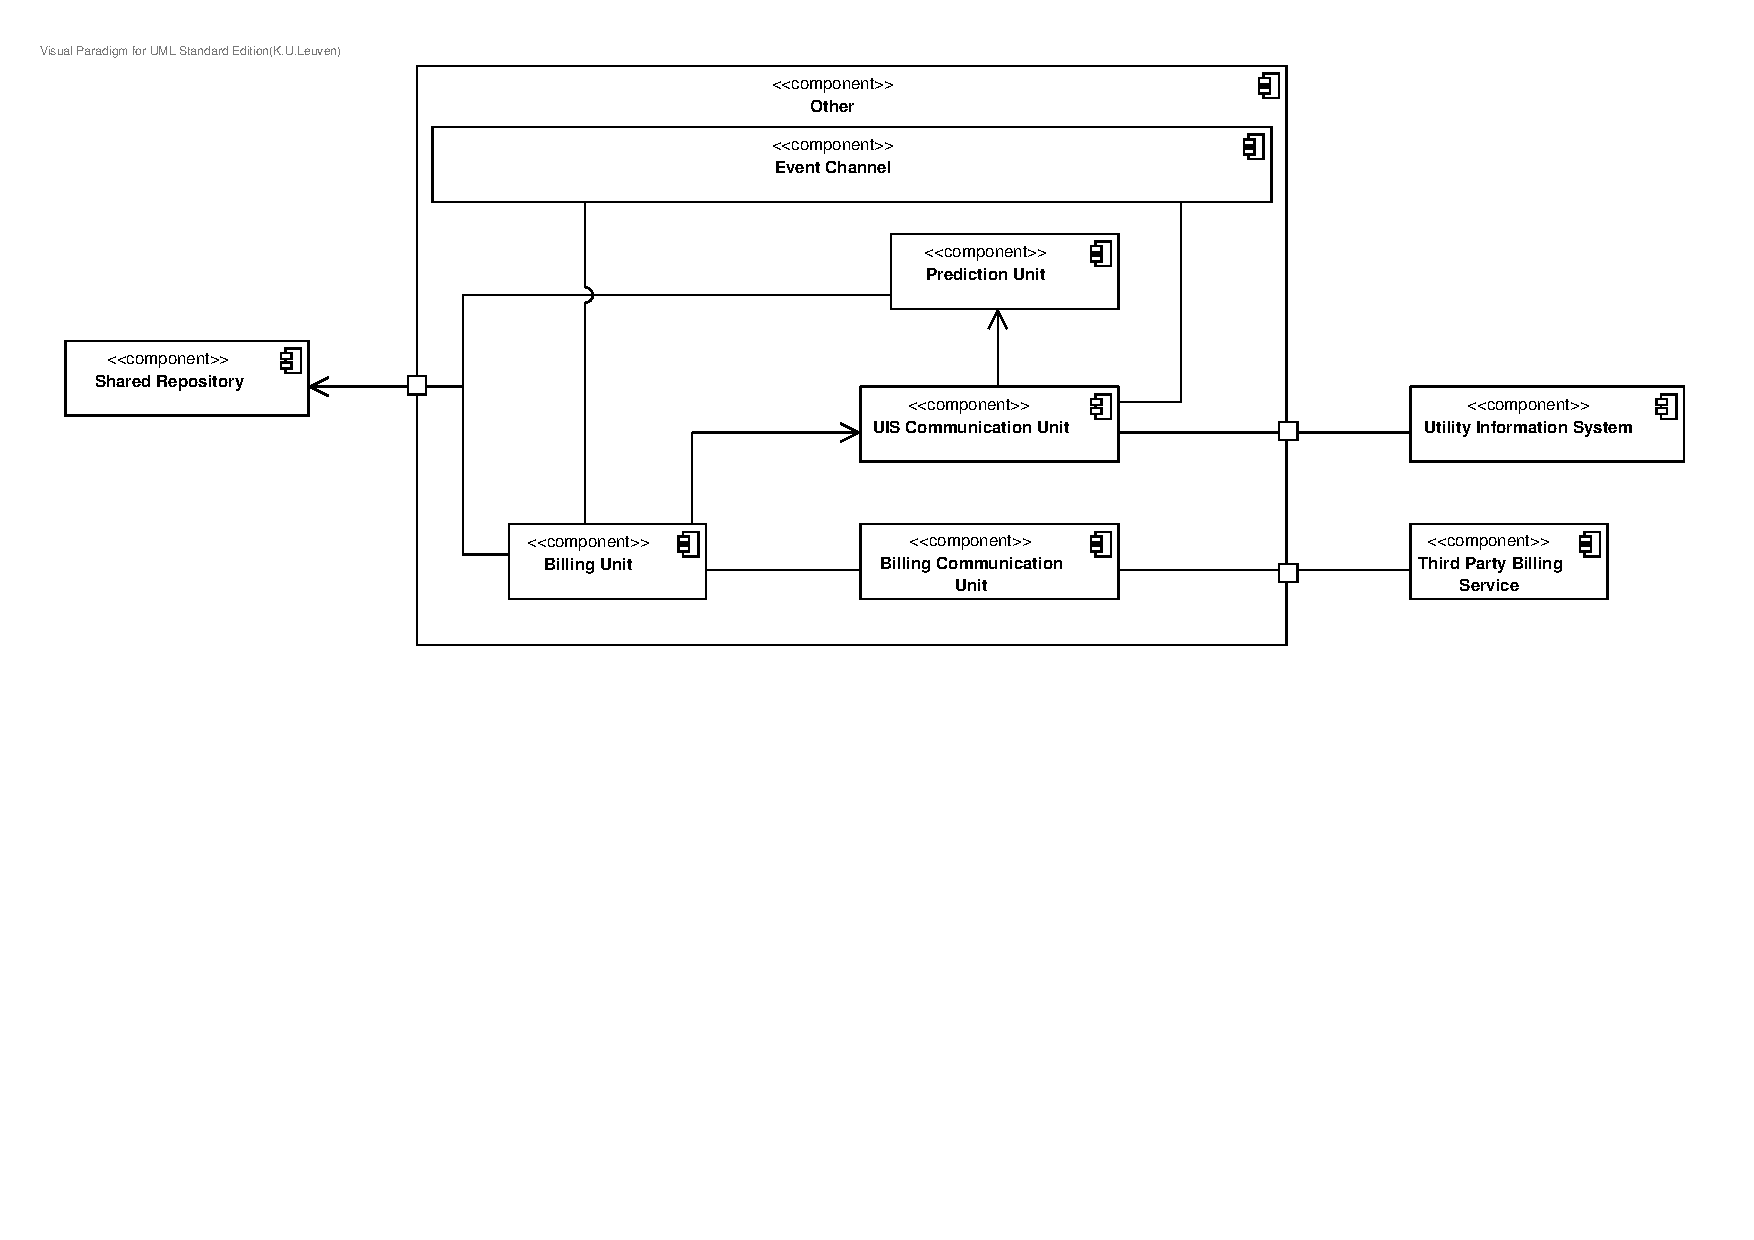
\includegraphics[width=\textwidth]{figs/add-it10-elements.pdf}
		\caption{Overview of the instantiated child elements in the other component}
		\label{fig:add/it10/decomposition}
	\end{centering}
\end{figure}

\npar The full decomposition of this iteration can be viewed in figure
\ref{fig:add/it10/decomposition}. In the subsection below each of the components
will be discussed. 

\subsubsection{PriceChannel}

\npar The PriceChannel is a communication entity where publishers can publish
events on and subscribers can subscribe on. Its solely goal is to redirect
incoming events to the right receivers. Notice that this component is only used
for the propagation of pricing updates.

\subsubsection{PredictionUnit}

\npar The PredictionUnit is responsible for fetching the consumption
histories of all customers and processing them (i.e. running all sorts of
prediction algorithms on the fetched data). The UISCommunicationUnit can
afterwards contact this component to retrieve the computed predictions.
Predictions are also made persistent in the Shared Repository.

\subsubsection{BillingUnit}

\npar The responsibility of this unit is limited to the generation of invoices.
This includes determining that an invoice should be constructed, fetching all
the relevant consumption data and constructing the invoice. The constructed
invoice is then sent towards the BillingCommunicationUnit through the
\interface{BillingSendAPI} interface. One more task is assigned to this
component, namely the marking of paid invoices. To retrieve all the data the
BillingUnit needs, first of all it has to have access to the internal ReMeS
customer database (through the \interface{CustomerProfileAPI} interface).
Secondly, it needs to be able to contact the UIS. This is done through the
\interface{CustomerInformation} interface.

\subsubsection{UISCommunicationUnit}

\npar This unit is the first of two units responsible for communication with
external actors in respect to billing and prediction. In section
\ref{add:it10/patterns} we discussed the usage of a slight variant of the
\emph{Facade} pattern. The deviation of the standard pattern lies firstly in the
usage of two communication units instead of one single point of access.
Secondly there is no bypassing of this communication (not even in a limited
number of scenarios) as it is the case in the \emph{Facade} pattern.

\npar This component interacts with three other components. The first one,
Utility information system, is used for all information needed by ReMeS that is
stored by the utility company. The second one, PredictionUnit, is used to
acquire prediction statistics for a certain utility company. Besides using
interfaces, the UISCommunicationUnit off course offers interfaces itself. It
offers two main services towards other components: one towards the BillingUnit
and one towards the UIS. The former service includes the retrieval of customer
data that is kept by the UIS. The latter one is more of a consultation service
where the UIS can request predictions.

\subsubsection{BillingCommunicationUnit}

\npar The responsibility of this unit is the handling of all information between
ReMeS and external actors regarding billing. It has two major duties. The first
is to allow invoices to be sent towards the third party billing service after
the invoice has been constructed off course. The second task is to provide a
possibility for all notifications that need to be sent towards ReMeS concerning
the payment of invoices.

\npar The BillingCommunicationUnit also uses functionality which is reflected in
the usage of the BillingUnit and Third Party Billing Service. The former one is
used to sent the notification of a payment to. It uses the Third Party Billing
Service for sending it the right documents.

\subsubsection{Portal}

\npar The Portal represents the web interface that is exposed to ReMeS users.
This includes customers, utility providers, ReMeS personnel\ldots

\npar Upon subscribing to ReMeS, the user receives a login with which he/she can
login and manage its profile, meters and utility usage. 

\subsection{Step 4: Define interfaces for instantiated elements}
\label{add:it10/interfaces}

\npar In this section each interface is explained in terms of the components
which use and/or offer it together with information about what is exchanged. For
detailed information with reference to the specific methods the interfaces
implement, we refer to the interface catalog, see appendix
\ref{chap:interface-catalog}.

\subsubsection{PriceChannelAPI}

\npar This interface is declared between the users of PriceChannel and the
implementor, PriceChannel itself. Events are dispatched through the channel
(and hence the interface) towards the subscribers.

\subsubsection{PredictionAPI}

\npar The \interface{PredictionAPI} interface is offered by the PredictionUnit
towards the UISCommunicationUnit. The latter can use this to send predictions to
whoever needs them.

\subsubsection{BillingUnitAPI}

\npar \interface{BillingUnitAPI} is an interface between the BillingUnit and the
BillingCommunicationUnit. It is used to notify the BillingUnit of payment of a
certain invoice.

\subsubsection{BillingCommunicationAPI}

\npar This interface has exactly the same role as the \interface{BillingUnitAPI}
but it is declared between the BillingCommunicationAPI on one side and the Third
Party Billing Service on the other side.

\subsubsection{CustomerInformation}

\npar The \interface{CustomerInformation} is situated between the BillingUnit
and the UISCommunicationUnit. Through this interface is customer information
exchanged.

\subsubsection{UISCommunicationAPI}

\npar This interface is declared between the UISCommunicationUnit, which
also offers the interface, and the UIS. This interface provides several services
to the UIS including prediction of utilities.

\subsubsection{BillingSendAPI}

\npar This interface is analogous to \interface{BillingCommunicationAPI}, but it
is declared between different components, namely the BillingCommunicationUnit
and the BillingUnit. The latter is the one who provides the interface.

\begin{figure}[H]
	\begin{centering}
		% TODO Figure 
		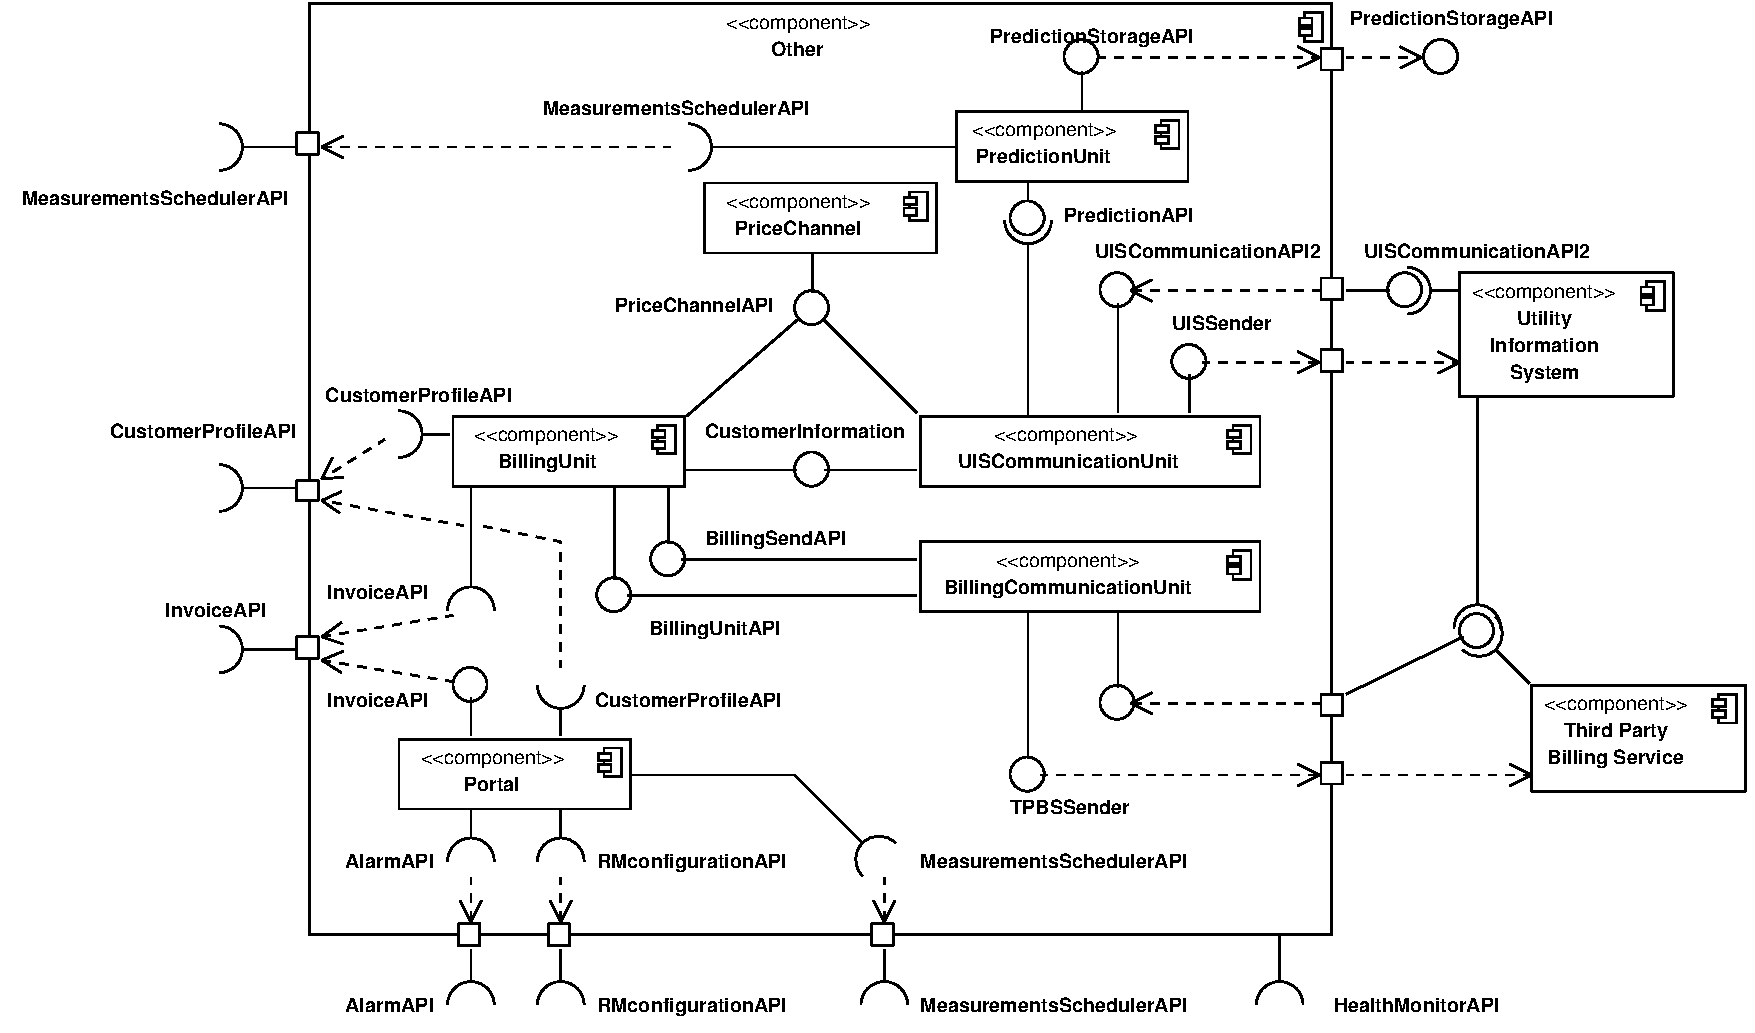
\includegraphics[width=\textwidth]{figs/add-it10-interfaces.pdf}
		\caption{Overview of the interfaces and components in the Other Component}
		\label{fig:it10/interfaces}
	\end{centering}
\end{figure}

\subsection{Step 5: Verify and refine}
\label{add:it10/verification}

\npar All quality attribute drivers and assigned use cases were resolved in
this iteration. 

\npar Use case 14 (request consumption predictions) is divided across the
UISCommunicationUnit and the PredictionUnit.

\npar The Billing Unit and Billing Communication are responsible for:

\begin{itemize}
    \item UC15: Generate invoice
    \item UC16: Mark invoice paid
\end{itemize}

\npar The following use cases are assigned to the ReMeS Portal.

\begin{itemize}
	\item UC1: Log in
	\item UC2: Log off
	\item UC3: Register customer
	\item UC4: Unregister customer
	\item UC5: Associate device to customer
	\item UC6: Customize customer profile
	\item UC11: Operate actuator remotely
	\item UC12: Set alarm recipients
	\item UC17': Perform Research
\end{itemize}